The distribution network used for testing the coordinated voltage control algorithm is the test system number 2, available under the SUNGRIN project \cite{SG}. This test system was obtained by reducing the network of a larger feeder and it represents a real system in the state of Florida. Fig. \ref{fig:Feeder2} \cite{SG} depicts the topology of the network. The tests were performed considering a balanced system, making it a 9 bus test system. The data for the loads and the PV profiles were also obtained from the SUNGRIN project for that specific location. Fig. \ref{fig:pv_data} shows the real power generation of the three PVs present in the system. The used profile data has a resolution of one minute. Table \ref{tab:load_data} represents the rated values of the loads in the system. Table \ref{tab:Inv_rate} presents the rating of the inverters connected to the PV systems. The inverter reactive power limits (Q limits) are determined by considering a maximum of 0.8 power factor at the point of common coupling. 

\begin{figure}[!h]
\centering
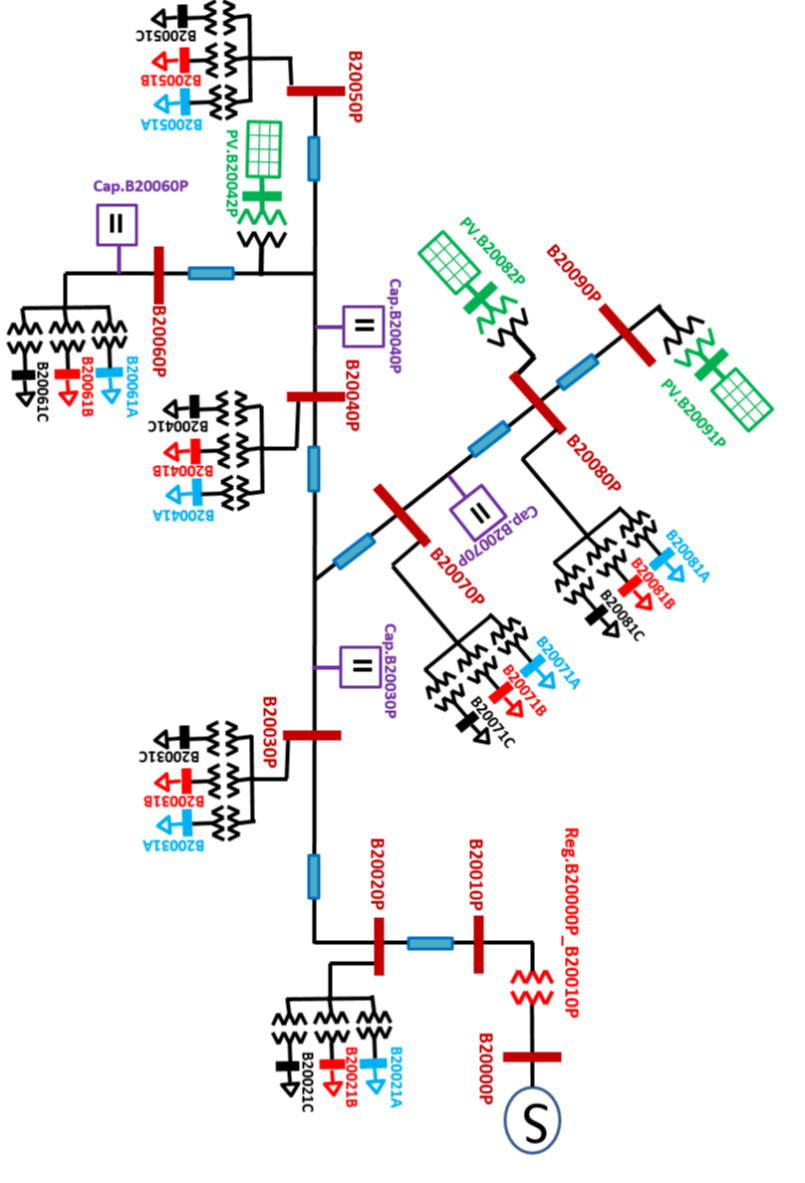
\includegraphics[width=0.85\linewidth]{figs/CVC/feeder_r.png}
\caption{Test Feeder Topology.}
\label{fig:Feeder2}
\end{figure}

\begin{figure}[!h]
\centering
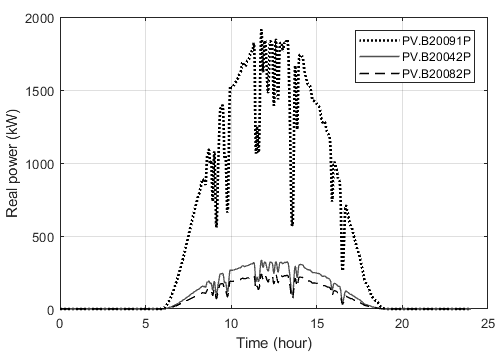
\includegraphics[width=\linewidth]{figs/CVC/PV_DATA.png}
\caption{Test Feeder Topology}
\label{fig:pv_data}
\end{figure}
% \begin{figure}[!h]
% \centering
% 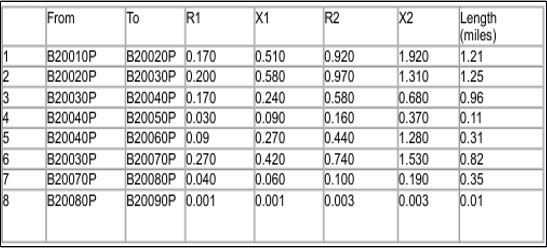
\includegraphics[width=7cm, height=3cm]{linedata.png}
% \caption{Line Data for the Distribution Network}
% \label{fig:BD1}
% \end{figure}

\begin{table}[!h]
\caption{Average load at nodes}
\label{tab:load_data}
\centering
\begin{tabular}{|c|c|c|}
\hline
Load & kVA & Power factor \\ \hline
B20020P & 1035 & 0.90 \\ \hline
B20030P & 2300 & 0.90 \\ \hline
B20040P & 1195 & 0.85 \\ \hline
B20050P & 225 & 0.85 \\ \hline
B20060P & 1285 & 0.85 \\ \hline
B20070P & 1365 & 0.85 \\ \hline
B20080P & 435 & 0.85 \\ \hline
\end{tabular}
\end{table}

% \begin{figure}[!h]
% \centering
% 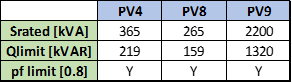
\includegraphics[width=6cm, height=2cm]{pvdata.png}
% \caption{PV Inverter Ratings}
% \label{fig:Inv_rate}
% \end{figure}

\begin{table}[!h]
\centering
\caption{PV Inverter Ratings}
\label{tab:Inv_rate}
\begin{tabular}{c|c|c|c|}
\cline{2-4}
 & PV.B20091P & PV.B20042P & PV.B20082P \\ \hline
\multicolumn{1}{|c|}{Rated power (kVA)} & 365 & 265 & 2200 \\ \hline
\multicolumn{1}{|c|}{Q limit (kVAR)} & 219 & 159 & 1320 \\ \hline
\end{tabular}
\end{table}